\documentclass[a4paper,11pt]{report}
\usepackage[showexo=true,showcorr=false]{../packages/coursclasse}
%Commenter ou enlever le commentaire sur la ligne suivante pour montrer le niveau
\toggletrue{montrerNiveaux}
%permet de gérer l'espacement entre les items des env enumerate et enumitem
\usepackage{enumitem}
\setlist[enumerate]{align=left,leftmargin=1cm,itemsep=10pt,parsep=0pt,topsep=0pt,rightmargin=0.5cm}
\setlist[itemize]{align=left,labelsep=1em,leftmargin=*,itemsep=0pt,parsep=0pt,topsep=0pt,rightmargin=0cm}
%permet de gerer l'espacement entre les colonnes de multicols
\setlength\columnsep{35pt}
\begin{document}
%%%%%%%%%%%%%%%%% À MODIFIER POUR CHAQUE SERIE %%%%%%%%%%%%%%%%%%%%%%%%%%%%%
\newcommand{\chapterName}{Fonctions et algèbre}
\newcommand{\serieName}{Propriétés de la proportionnalité}


%%%%%%%%%%%%%%%%%% PREMIERE PAGE NE PAS MODIFER %%%%%%%%%%%%%%%%%%%%%%%%
% le chapitre en cours, ne pas changer au cours d'une série
\chapter*{\chapterName}
\thispagestyle{empty}

%%%%% LISTE AIDE MEMOIRE %%%%%%
\begin{amL}{\serieName}{
\item Généralités (page 55)
\item Résoudre un problème de proportionnalité (page 57)}
\end{amL}
%%%%%%%%%%%%%%% DEBUT DE LA SERIE NE PAS MODIFIER %%%%%%%%%%%%%%%%%%%%%%%%%%%%%
\section*{\serieName}
\setcounter{page}{1}
\thispagestyle{firstPage}



%%%%%%%%%%% LES EXERCICES %%%%%%%%%%%%%%%%%%%%%%%%%%%%%%%%%%%
\begin{resolu}{Avec le coefficient}{Complète le tableau de proportionnalité ci-dessous avec le coefficient de proportionnalité.
	\vspace{-0.3cm}
\begin{center}
	\psfrag{a}{Pommes (\tunit{}{\kg})}
	\psfrag{b}{Prix à payer (\tunit{}{\fr})}
\psfrag{c}[c][c]{2}
\psfrag{d}[c][c]{6}
\psfrag{e}[c][c]{4}
\psfrag{f}[c][c]{}
\psfrag{g}[c][c]{5}
\psfrag{h}[c][c]{}
\psfrag{i}[c][c]{}
\psfrag{j}[c][c]{21}
\psfrag{k}[c][c]{}
\psfrag{l}[c][c]{33}
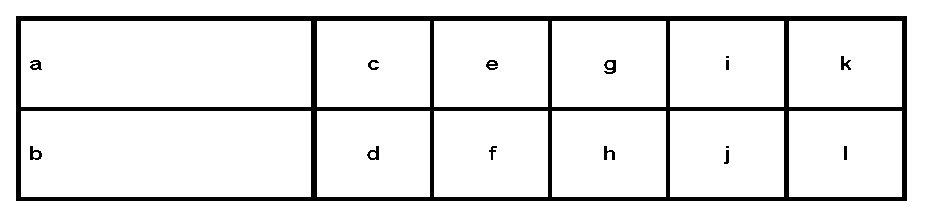
\includegraphics[scale=.9]{media/fa-30/tableaun.eps}
\end{center}
{\color{blue}
Pour calculer le coefficient, on doit effectuer la division suivante~: 

$6\div2 ={\color{blue}3}.$

	\vspace{-0.8cm}
\begin{center}
	\psfrag{a}{Pommes (\tunit{}{\kg})}
	\psfrag{b}{Prix à payer (\tunit{}{\fr})}
\psfrag{c}[c][c]{2}
\psfrag{d}[c][c]{6}
\psfrag{e}[c][c]{4}
\psfrag{f}[c][c]{\color{brown}12}
\psfrag{g}[c][c]{5}
\psfrag{h}[c][c]{\color{brown}15}
\psfrag{i}[c][c]{}
\psfrag{j}[c][c]{21}
\psfrag{k}[c][c]{}
\psfrag{l}[c][c]{33}
\psfrag{m}[c][c]{{\Large\color{brown}$\cdot$} {\color{blue}3}}
\includegraphics[scale=.9]{media/fa-30/tableaucoeffn.eps}
\end{center}
Ainsi pour obtenir les deux valeurs en brun , on a effectué respectivement les calculs $$ 4 {\color{brown}\cdot} {\color{blue}3}= {\color{brown}12} \quad\mbox{et}\quad 5 {\color{brown}\cdot} {\color{blue}3}= {\color{brown}15}$$

\vspace{-0.5cm}
\begin{center}
	\psfrag{a}{Pommes (\tunit{}{\kg})}
	\psfrag{b}{Prix à payer (\tunit{}{\fr})}
\psfrag{c}[c][c]{2}
\psfrag{d}[c][c]{6}
\psfrag{e}[c][c]{4}
\psfrag{f}[c][c]{\color{brown}12}
\psfrag{g}[c][c]{5}
\psfrag{h}[c][c]{\color{brown}15}
\psfrag{i}[c][c]{\color{red}7}
\psfrag{j}[c][c]{21}
\psfrag{k}[c][c]{\color{red}11}
\psfrag{l}[c][c]{33}
\psfrag{m}[c][c]{{\Large\color{red}$\div$} {\color{blue}3}}
\includegraphics[scale=.9]{media/fa-30/tableaucoeff2n.eps}
\end{center}
Et pour trouver les deux valeurs en rouge, on  a effectué respectivement les calculs $$21 {\color{red}\div} {\color{blue} 3} = {\color{red} 7} \quad\mbox{et}\quad 33 {\color{red}\div} {\color{blue} 3} = {\color{red} 11} .$$
}}{1}
\end{resolu}


\begin{exop}{
Complète le tableau de proportionnalité ci-dessous à l'aide de la méthode du coefficient de proportionnalité.
 
\vspace{-0.8cm}
\begin{center}
	\psfrag{a}{Abricots (\tunit{}{\kg})}
	\psfrag{b}{Prix à payer (\tunit{}{\fr})}
\psfrag{c}[c][c]{2}
\psfrag{d}[c][c]{12}
\psfrag{e}[c][c]{5}
\psfrag{f}[c][c]{}
\psfrag{g}[c][c]{8}
\psfrag{h}[c][c]{}
\psfrag{i}[c][c]{}
\psfrag{j}[c][c]{72}
\psfrag{k}[c][c]{}
\psfrag{l}[c][c]{90}
\psfrag{m}[c][c]{\Large\color{brown}{$\cdot \qquad$}}
\includegraphics[scale=.9]{media/fa-30/tableaucoeffn.eps}
\end{center}
\vspace{-0.5cm}}{1}
\end{exop}


\begin{exop}{
Complète le tableau de proportionnalité ci-dessous à l'aide de la méthode du coefficient de proportionnalité.
 

\vspace{-0.8cm}
\begin{center}
\psfrag{a}{Grandeur 1}
\psfrag{b}{Grandeur 2}
\psfrag{c}[c][c]{1}
\psfrag{d}[c][c]{}
\psfrag{e}[c][c]{3}
\psfrag{f}[c][c]{21}
\psfrag{g}[c][c]{5}
\psfrag{h}[c][c]{}
\psfrag{i}[c][c]{}
\psfrag{j}[c][c]{49}
\psfrag{k}[c][c]{}
\psfrag{l}[c][c]{63}
\psfrag{m}[c][c]{\Large\color{brown}{$\cdot \qquad$}}
\includegraphics[scale=.9]{media/fa-30/tableaucoeffn.eps}
\end{center}
\vspace{-0.5cm}}{1}
\end{exop}

\begin{exop}{
Complète le tableau de proportionnalité ci-dessous à l'aide de la méthode du coefficient de proportionnalité.
 
	\vspace{-0.8cm}
\begin{center}
\psfrag{a}{Grandeur 1}
\psfrag{b}{Grandeur 2}
\psfrag{c}[c][c]{1}
\psfrag{d}[c][c]{}
\psfrag{e}[c][c]{}
\psfrag{f}[c][c]{60}
\psfrag{g}[c][c]{}
\psfrag{h}[c][c]{84}
\psfrag{i}[c][c]{10}
\psfrag{j}[c][c]{}
\psfrag{k}[c][c]{11}
\psfrag{l}[c][c]{132}
\psfrag{m}[c][c]{\Large\color{brown}{$\cdot \qquad$}}
\includegraphics[scale=.9]{media/fa-30/tableaucoeffn.eps}
\end{center}
\vspace{-0.5cm}}{1}
\end{exop}

\newpage
\begin{exop}
{Complète le tableau de proportionnalité ci-dessous à l'aide de la méthode du coefficient de proportionnalité.
 
	\vspace{-0.8cm}
\begin{center}
	\psfrag{a}{Fraises (\tunit{}{\kg})}
	\psfrag{b}{Prix à payer (\tunit{}{\fr})}
\psfrag{c}[c][c]{}
\psfrag{d}[c][c]{2}
\psfrag{e}[c][c]{54}
\psfrag{f}[c][c]{}
\psfrag{g}[c][c]{63}
\psfrag{h}[c][c]{}
\psfrag{i}[c][c]{}
\psfrag{j}[c][c]{9}
\psfrag{k}[c][c]{90}
\psfrag{l}[c][c]{10}
\psfrag{m}[c][c]{\Large\color{brown}{$\cdot \qquad$}}
\includegraphics[scale=.9]{media/fa-30/tableaucoeffn.eps}
\end{center}
\vspace{-0.5cm}}{1}
\end{exop}

\begin{exop}{
Complète le tableau de proportionnalité ci-dessous à l'aide de la méthode du coefficient de proportionnalité.
 
	\vspace{-0.8cm}
\begin{center}
\psfrag{a}{Grandeur 1}
\psfrag{b}{Grandeur 2}
\psfrag{c}[c][c]{5}
\psfrag{d}[c][c]{2}
\psfrag{e}[c][c]{}
\psfrag{f}[c][c]{5}
\psfrag{g}[c][c]{15}
\psfrag{h}[c][c]{}
\psfrag{i}[c][c]{}
\psfrag{j}[c][c]{7}
\psfrag{k}[c][c]{22,5}
\psfrag{l}[c][c]{}
\psfrag{m}[c][c]{\Large\color{brown}{$\cdot \qquad$}}
\includegraphics[scale=.9]{media/fa-30/tableaucoeffn.eps}
\end{center}
\vspace{-0.5cm}}{1}
\end{exop}


\begin{exop}{
Complète le tableau de proportionnalité ci-dessous à l'aide de la méthode du coefficient de proportionnalité.
 
	\vspace{-0.8cm}
\begin{center}
\psfrag{a}{Grandeur 1}
\psfrag{b}{Grandeur 2}
\psfrag{c}[c][c]{}
\psfrag{d}[c][c]{2}
\psfrag{e}[c][c]{}
\psfrag{f}[c][c]{3}
\psfrag{g}[c][c]{44}
\psfrag{h}[c][c]{4}
\psfrag{i}[c][c]{121}
\psfrag{j}[c][c]{}
\psfrag{k}[c][c]{132}
\psfrag{l}[c][c]{}
\psfrag{m}[c][c]{\Large\color{brown}{$\cdot \qquad$}}
\includegraphics[scale=.9]{media/fa-30/tableaucoeffn.eps}
\end{center}
\vspace{-0.5cm}}{1}
\end{exop}







\newpage
\begin{resolu}{Avec la propriété du produit}{Complète le tableau de proportionnalité ci-dessous avec la propriété du produit.

\begin{center}
\psfrag{a}{Nb de stylos }
\psfrag{b}{Prix à payer (\tunit{}{\fr})}
\psfrag{c}[c][c]{2}
\psfrag{d}[c][c]{5}
\psfrag{e}[c][c]{8}
\psfrag{f}[c][c]{\color{brown}20}
\psfrag{g}[c][c]{24}
\psfrag{h}[c][c]{\color{red}60}
\psfrag{i}[c][c]{\color{blue}20}
\psfrag{j}[c][c]{50}
\psfrag{k}[c][c]{40}
\psfrag{l}[c][c]{100}
\psfrag{m}[c][c]{{\Large\color{brown}$\cdot$ 4}}
\psfrag{n}[c][c]{{\Large\color{brown}$\cdot$ 3}}
\psfrag{o}[c][c]{{\Large\color{blue}$\div$ 2}}
\includegraphics[scale=.9]{media/fa-30/tableaufractionn.eps}
\end{center}
}{1}
\end{resolu}



\begin{exop}{
Complète le tableau de proportionnalité ci-dessous à l'aide de la propriété du produit.
\begin{center}
\psfrag{a}{Nb de stylos}
\psfrag{b}{Prix à payer (\tunit{}{\fr})}
\psfrag{c}[c][c]{2}
\psfrag{d}[c][c]{7}
\psfrag{e}[c][c]{4}
\psfrag{f}[c][c]{}
\psfrag{g}[c][c]{}
\psfrag{h}[c][c]{21}
\psfrag{i}[c][c]{}
\psfrag{j}[c][c]{84}
\psfrag{k}[c][c]{18}
\psfrag{l}[c][c]{}
\psfrag{m}[c][c]{9}
\psfrag{n}[c][c]{}
\includegraphics[scale=.9]{media/fa-30/tableaut.eps}
\end{center}
\vspace{-0.5cm}}{1}
\end{exop}
\begin{exop}{
Complète le tableau de proportionnalité ci-dessous à l'aide de la propriété du produit.
\begin{center}
\psfrag{a}{Nb de cahiers}
\psfrag{b}{Prix à payer (\tunit{}{\fr})}
\psfrag{c}[c][c]{2}
\psfrag{d}[c][c]{}
\psfrag{e}[c][c]{}
\psfrag{f}[c][c]{15}
\psfrag{g}[c][c]{6}
\psfrag{h}[c][c]{30}
\psfrag{i}[c][c]{}
\psfrag{j}[c][c]{90}
\psfrag{k}[c][c]{12}
\psfrag{l}[c][c]{}
\psfrag{m}[c][c]{}
\psfrag{n}[c][c]{100}
\includegraphics[scale=.9]{media/fa-30/tableaut.eps}
\end{center}
\vspace{-0.5cm}}{1}
\end{exop}
\begin{exop}{
Complète le tableau de proportionnalité ci-dessous à l'aide de la propriété du produit.
\begin{center}
\psfrag{a}{Grandeur 1}
\psfrag{b}{Grandeur 2}
\psfrag{c}[c][c]{3}
\psfrag{d}[c][c]{11}
\psfrag{e}[c][c]{}
\psfrag{f}[c][c]{22}
\psfrag{g}[c][c]{}
\psfrag{h}[c][c]{55}
\psfrag{i}[c][c]{18}
\psfrag{j}[c][c]{}
\psfrag{k}[c][c]{36}
\psfrag{l}[c][c]{}
\psfrag{m}[c][c]{}
\psfrag{n}[c][c]{33}
\includegraphics[scale=.9]{media/fa-30/tableaut.eps}
\end{center}
\vspace{-0.5cm}}{1}
\end{exop}

\begin{exop}{
Complète le tableau de proportionnalité ci-dessous à l'aide de la propriété du produit.
\begin{center}
\psfrag{a}{Grandeur 1}
\psfrag{b}{Grandeur 2}
\psfrag{c}[c][c]{7}
\psfrag{d}[c][c]{4}
\psfrag{e}[c][c]{}
\psfrag{f}[c][c]{8}
\psfrag{g}[c][c]{28}
\psfrag{h}[c][c]{}
\psfrag{i}[c][c]{49}
\psfrag{j}[c][c]{}
\psfrag{k}[c][c]{}
\psfrag{l}[c][c]{40}
\psfrag{m}[c][c]{}
\psfrag{n}[c][c]{48}
\includegraphics[scale=.9]{media/fa-30/tableaut.eps}
\end{center}
\vspace{-0.5cm}}{1}
\end{exop}
\begin{exop}{
Complète le tableau de proportionnalité ci-dessous à l'aide de la propriété du produit.
\begin{center}
\psfrag{a}{Grandeur 1}
\psfrag{b}{Grandeur 2}
\psfrag{c}[c][c]{9}
\psfrag{d}[c][c]{}
\psfrag{e}[c][c]{18}
\psfrag{f}[c][c]{10}
\psfrag{g}[c][c]{}
\psfrag{h}[c][c]{20}
\psfrag{i}[c][c]{}
\psfrag{j}[c][c]{25}
\psfrag{k}[c][c]{54}
\psfrag{l}[c][c]{}
\psfrag{m}[c][c]{90}
\psfrag{n}[c][c]{}
\includegraphics[scale=.9]{media/fa-30/tableaut.eps}
\end{center}
\vspace{-0.5cm}}{1}
\end{exop}
\begin{exop}{
Complète le tableau de proportionnalité ci-dessous à l'aide de la propriété du produit.
\begin{center}
\psfrag{a}{Grandeur 1}
\psfrag{b}{Grandeur 2}
\psfrag{c}[c][c]{2}
\psfrag{d}[c][c]{3}
\psfrag{e}[c][c]{}
\psfrag{f}[c][c]{15}
\psfrag{g}[c][c]{24}
\psfrag{h}[c][c]{}
\psfrag{i}[c][c]{6}
\psfrag{j}[c][c]{}
\psfrag{k}[c][c]{}
\psfrag{l}[c][c]{6}
\psfrag{m}[c][c]{}
\psfrag{n}[c][c]{72}
\includegraphics[scale=.9]{media/fa-30/tableaut.eps}
\end{center}
\vspace{-0.5cm}}{1}
\end{exop}





\begin{resolu}{Propriété de la somme}{Complète le tableau ci-dessous à l'aide de la propriété de la somme pour une recette d'un gâteau au chocolat où l'on indique la quantité de farine en fonction du nombre de personnes.

\vspace*{1cm}
\begin{center}
\psfrag{a}{Nb de personnes }
\psfrag{b}{Farine (\tunit{}{\g})}
\psfrag{c}[c][c]{4}
\psfrag{d}[c][c]{100}
\psfrag{e}[c][c]{\color{blue}5}
\psfrag{f}[c][c]{125}
\psfrag{g}[c][c]{6}
\psfrag{h}[c][c]{150}
\psfrag{i}[c][c]{7}
\psfrag{j}[c][c]{175}
\psfrag{k}[c][c]{10}
\psfrag{l}[c][c]{\color{red}250}
\psfrag{m}[c][c]{12}
\psfrag{n}[c][c]{300}
%\psfrag{o}[c][c]{}
\psfrag{p}[c][c]{\color{red}$+$}
\psfrag{q}[c][c]{\color{red}$=$}
\psfrag{r}[c][c]{\color{blue}$=$}
\psfrag{s}[c][c]{\color{blue}$-$}
\includegraphics[scale=.9]{media/fa-30/tableauaddn.eps}
\end{center}
\vspace*{1cm}
}{1}
\end{resolu}










\begin{exop}{
Complète le tableau de proportionnalité ci-dessous à l'aide de la propriété de la somme.
\begin{center}
\psfrag{a}{Nectarines (\tunit{}{\kg}) }
\psfrag{b}{Prix à payer (\tunit{}{\fr})}
\psfrag{c}[c][c]{2}
\psfrag{d}[c][c]{9}
\psfrag{e}[c][c]{5}
\psfrag{f}[c][c]{22,5}
\psfrag{g}[c][c]{7}
\psfrag{h}[c][c]{}
\psfrag{i}[c][c]{}
\psfrag{j}[c][c]{54}
\psfrag{k}[c][c]{10}
\psfrag{l}[c][c]{}
\psfrag{m}[c][c]{14}
\psfrag{n}[c][c]{}
\includegraphics[scale=.9]{media/fa-30/tableaut.eps}
\end{center}
\vspace{-0.5cm}}{1}
\end{exop}
\begin{exop}{
Complète le tableau de proportionnalité ci-dessous à l'aide de la propriété de la somme.
\begin{center}
\psfrag{a}{Nb de places}
\psfrag{b}{Prix à payer (\tunit{}{\fr})}
\psfrag{c}[c][c]{2}
\psfrag{d}[c][c]{50}
\psfrag{e}[c][c]{3}
\psfrag{f}[c][c]{75}
\psfrag{g}[c][c]{4}
\psfrag{h}[c][c]{100}
\psfrag{i}[c][c]{5}
\psfrag{j}[c][c]{}
\psfrag{k}[c][c]{}
\psfrag{l}[c][c]{150}
\psfrag{m}[c][c]{7}
\psfrag{n}[c][c]{}
\includegraphics[scale=.9]{media/fa-30/tableaut.eps}
\end{center}
\vspace{-0.5cm}}{1}
\end{exop}
\begin{exop}{
Complète le tableau de proportionnalité ci-dessous à l'aide de la propriété de la somme.
\begin{center}
\psfrag{a}{Grandeur 1}
\psfrag{b}{Grandeur 2}
\psfrag{c}[c][c]{1}
\psfrag{d}[c][c]{9,5}
\psfrag{e}[c][c]{2}
\psfrag{f}[c][c]{19}
\psfrag{g}[c][c]{}
\psfrag{h}[c][c]{28,5}
\psfrag{i}[c][c]{5}
\psfrag{j}[c][c]{}
\psfrag{k}[c][c]{8}
\psfrag{l}[c][c]{78}
\psfrag{m}[c][c]{10}
\psfrag{n}[c][c]{}
\includegraphics[scale=.9]{media/fa-30/tableaut.eps}
\end{center}
\vspace{-0.5cm}}{1}
\end{exop}

\begin{exop}{
Complète le tableau de proportionnalité ci-dessous à l'aide de la propriété de la somme.
\begin{center}
\psfrag{a}{Grandeur 1}
\psfrag{b}{Grandeur 2}
\psfrag{c}[c][c]{4}
\psfrag{d}[c][c]{5}
\psfrag{e}[c][c]{6}
\psfrag{f}[c][c]{}
\psfrag{g}[c][c]{10}
\psfrag{h}[c][c]{12,5}
\psfrag{i}[c][c]{14}
\psfrag{j}[c][c]{}
\psfrag{k}[c][c]{16}
\psfrag{l}[c][c]{}
\psfrag{m}[c][c]{}
\psfrag{n}[c][c]{37,5}
\includegraphics[scale=.9]{media/fa-30/tableaut.eps}
\end{center}
\vspace{-0.5cm}}{1}
\end{exop}

\begin{exop}{
Complète le tableau de proportionnalité ci-dessous à l'aide de la propriété de la somme.
\begin{center}
\psfrag{a}{Grandeur 1}
\psfrag{b}{Grandeur 2}
\psfrag{c}[c][c]{7}
\psfrag{d}[c][c]{3}
\psfrag{e}[c][c]{21}
\psfrag{f}[c][c]{9}
\psfrag{g}[c][c]{}
\psfrag{h}[c][c]{12}
\psfrag{i}[c][c]{}
\psfrag{j}[c][c]{21}
\psfrag{k}[c][c]{14}
\psfrag{l}[c][c]{6}
\psfrag{m}[c][c]{}
\psfrag{n}[c][c]{27}
\includegraphics[scale=.9]{media/fa-30/tableaut.eps}
\end{center}
\vspace{-0.5cm}}{1}
\end{exop}

\begin{resolu}
{Retour à l'unité}{Complète la tableau de proportionnalité ci-dessous à l'aide du retour à l'unité.
\begin{center}
\psfrag{a}{Kiwis (pièces)}
\psfrag{b}{Prix à payer (\tunit{}{\fr})}
\psfrag{c}[c][c]{5}
\psfrag{d}[c][c]{6}
\psfrag{e}[c][c]{7}
\psfrag{f}[c][c]{}
\psfrag{g}[c][c]{9}
\psfrag{h}[c][c]{}
\psfrag{i}[c][c]{13}
\psfrag{j}[c][c]{}
\psfrag{k}[c][c]{17}
\psfrag{l}[c][c]{}
\psfrag{m}[c][c]{}
\psfrag{n}[c][c]{}
\includegraphics[scale=.9]{media/fa-30/tableaut.eps}
\end{center}

{\color{blue}
On commence par calculer le prix d'un kiwi~: $6 \div 5 = 1,\!2.$ Puis, on complète la dernière colonne.}
\begin{center}
\psfrag{a}{Kiwis (pièces)}
\psfrag{b}{Prix à payer (\tunit{}{\fr})}
\psfrag{c}[c][c]{5}
\psfrag{d}[c][c]{6}
\psfrag{e}[c][c]{7}
\psfrag{f}[c][c]{}
\psfrag{g}[c][c]{9}
\psfrag{h}[c][c]{}
\psfrag{i}[c][c]{13}
\psfrag{j}[c][c]{}
\psfrag{k}[c][c]{17}
\psfrag{l}[c][c]{}
\psfrag{m}[c][c]{{\color{blue} 1}}
\psfrag{n}[c][c]{{\color{blue} 1,2}}
\includegraphics[scale=.9]{media/fa-30/tableaut.eps}
\end{center}

{\color{blue}
Ensuite, on multiplie la valeur de l'unité (le prix d'un kiwi qui coûte 1,20 CHF) par la quantité recherchée. Ainsi, on peut faire les calculs suivants qui vont nous permettre de compléter le tableau~:
\begin{multicols}{2}
$7 \cdot 1,2 =8,\!4$

$9 \cdot 1,2 =10,\!8$

$13 \cdot 1,2 =15,\!6$

$17 \cdot 1,2 =20,\!4$
\end{multicols}

}
\begin{center}
\psfrag{a}{Kiwis (pièces)}
\psfrag{b}{Prix à payer (\tunit{}{\fr})}
\psfrag{c}[c][c]{5}
\psfrag{d}[c][c]{6}
\psfrag{e}[c][c]{7}
\psfrag{f}[c][c]{{\color{blue} 8,4}}
\psfrag{g}[c][c]{9}
\psfrag{h}[c][c]{{\color{blue} 10,8}}
\psfrag{i}[c][c]{13}
\psfrag{j}[c][c]{{\color{blue} 15,6}}
\psfrag{k}[c][c]{17}
\psfrag{l}[c][c]{{\color{blue} 20,4}}
\psfrag{m}[c][c]{{\color{blue} 1}}
\psfrag{n}[c][c]{{\color{blue} 1,2}}
\includegraphics[scale=.9]{media/fa-30/tableaut.eps}
\end{center}




}{1}
\end{resolu}

\newpage
\begin{exop}{
Complète le tableau de proportionnalité ci-dessous à l'aide du retour à l'unité.
\begin{center}
\psfrag{a}{Nb de tartelettes}
\psfrag{b}{Prix à payer (\tunit{}{\fr})}
\psfrag{c}[c][c]{9}
\psfrag{d}[c][c]{36}
\psfrag{e}[c][c]{11}
\psfrag{f}[c][c]{}
\psfrag{g}[c][c]{20}
\psfrag{h}[c][c]{}
\psfrag{i}[c][c]{35}
\psfrag{j}[c][c]{}
\psfrag{k}[c][c]{40}
\psfrag{l}[c][c]{}
\psfrag{m}[c][c]{{\color{blue}1}}
\psfrag{n}[c][c]{}
\includegraphics[scale=.9]{media/fa-30/tableaut.eps}
\end{center}
\vspace{-0.5cm}}{1}
\end{exop}


\begin{exop}{
Complète le tableau de proportionnalité ci-dessous à l'aide du retour à l'unité.
\begin{center}
\psfrag{a}{Nb de kiwis}
\psfrag{b}{Prix à payer (\tunit{}{\fr})}
\psfrag{c}[c][c]{8}
\psfrag{d}[c][c]{12}
\psfrag{e}[c][c]{10}
\psfrag{f}[c][c]{}
\psfrag{g}[c][c]{15}
\psfrag{h}[c][c]{}
\psfrag{i}[c][c]{19}
\psfrag{j}[c][c]{}
\psfrag{k}[c][c]{23}
\psfrag{l}[c][c]{}
\psfrag{m}[c][c]{{\color{blue}1}}
\psfrag{n}[c][c]{}
\includegraphics[scale=.9]{media/fa-30/tableaut.eps}
\end{center}
\vspace{-0.5cm}}{1}
\end{exop}

\begin{exop}{
Complète le tableau de proportionnalité ci-dessous à l'aide du retour à l'unité.
\begin{center}
\psfrag{a}{Grandeur 1}
\psfrag{b}{Grandeur 2}
\psfrag{c}[c][c]{49}
\psfrag{d}[c][c]{14}
\psfrag{e}[c][c]{}
\psfrag{f}[c][c]{5}
\psfrag{g}[c][c]{}
\psfrag{h}[c][c]{8}
\psfrag{i}[c][c]{}
\psfrag{j}[c][c]{18}
\psfrag{k}[c][c]{}
\psfrag{l}[c][c]{22}
\psfrag{m}[c][c]{}
\psfrag{n}[c][c]{{\color{blue}1}}
\includegraphics[scale=.9]{media/fa-30/tableaut.eps}
\end{center}
\vspace{-0.5cm}}{1}
\end{exop}


\begin{exop}{
Complète le tableau de proportionnalité ci-dessous à l'aide du retour à l'unité.
\begin{center}
\psfrag{a}{Grandeur 1}
\psfrag{b}{Grandeur 2}
\psfrag{c}[c][c]{27}
\psfrag{d}[c][c]{12}
\psfrag{e}[c][c]{}
\psfrag{f}[c][c]{27}
\psfrag{g}[c][c]{}
\psfrag{h}[c][c]{13}
\psfrag{i}[c][c]{}
\psfrag{j}[c][c]{7}
\psfrag{k}[c][c]{}
\psfrag{l}[c][c]{5}
\psfrag{m}[c][c]{}
\psfrag{n}[c][c]{{\color{blue}1}}
\includegraphics[scale=.9]{media/fa-30/tableaut.eps}
\end{center}
\vspace{-0.5cm}}{1}
\end{exop}

\newpage
\begin{exop}{
Complète le tableau de proportionnalité ci-dessous à l'aide de la méthode de ton choix.
\begin{center}
\psfrag{a}{Grandeur 1}
\psfrag{b}{Grandeur 2}
\psfrag{c}[c][c]{6}
\psfrag{d}[c][c]{}
\psfrag{e}[c][c]{9}
\psfrag{f}[c][c]{21}
\psfrag{g}[c][c]{15}
\psfrag{h}[c][c]{}
\psfrag{i}[c][c]{}
\psfrag{j}[c][c]{63}
\psfrag{k}[c][c]{30}
\psfrag{l}[c][c]{}
\psfrag{m}[c][c]{}
\psfrag{n}[c][c]{84}
\includegraphics[scale=.9]{media/fa-30/tableaut.eps}
\end{center}
\vspace{-0.5cm}}{1}
\end{exop}

\begin{exop}{
Complète le tableau de proportionnalité ci-dessous à l'aide de la méthode de ton choix.
\begin{center}
\psfrag{a}{Grandeur 1}
\psfrag{b}{Grandeur 2}
\psfrag{c}[c][c]{4}
\psfrag{d}[c][c]{}
\psfrag{e}[c][c]{2}
\psfrag{f}[c][c]{}
\psfrag{g}[c][c]{6}
\psfrag{h}[c][c]{9}
\psfrag{i}[c][c]{}
\psfrag{j}[c][c]{15}
\psfrag{k}[c][c]{}
\psfrag{l}[c][c]{18}
\psfrag{m}[c][c]{14}
\psfrag{n}[c][c]{}
\includegraphics[scale=.9]{media/fa-30/tableaut.eps}
\end{center}
\vspace{-0.5cm}}{1}
\end{exop}

\begin{exop}{
Complète le tableau de proportionnalité ci-dessous à l'aide de la méthode de ton choix.
\begin{center}
\psfrag{a}{Grandeur 1}
\psfrag{b}{Grandeur 2}
\psfrag{c}[c][c]{3}
\psfrag{d}[c][c]{2}
\psfrag{e}[c][c]{9}
\psfrag{f}[c][c]{}
\psfrag{g}[c][c]{1,5}
\psfrag{h}[c][c]{}
\psfrag{i}[c][c]{7,5}
\psfrag{j}[c][c]{}
\psfrag{k}[c][c]{12}
\psfrag{l}[c][c]{}
\psfrag{m}[c][c]{16,5}
\psfrag{n}[c][c]{}
\includegraphics[scale=.9]{media/fa-30/tableaut.eps}
\end{center}
\vspace{-0.5cm}}{1}
\end{exop}

\begin{exop}{
Complète le tableau de proportionnalité ci-dessous à l'aide de la méthode de ton choix.
\begin{center}
\psfrag{a}{Grandeur 1}
\psfrag{b}{Grandeur 2}
\psfrag{c}[c][c]{0,2}
\psfrag{d}[c][c]{13}
\psfrag{e}[c][c]{0,4}
\psfrag{f}[c][c]{}
\psfrag{g}[c][c]{0,5}
\psfrag{h}[c][c]{32,5}
\psfrag{i}[c][c]{0,7}
\psfrag{j}[c][c]{}
\psfrag{k}[c][c]{5}
\psfrag{l}[c][c]{}
\psfrag{m}[c][c]{12}
\psfrag{n}[c][c]{}
\includegraphics[scale=.9]{media/fa-30/tableaut.eps}
\end{center}
\vspace{-0.5cm}}{1}
\end{exop}










%%%%%%%%%%%%%%%%%%%%%%%%%%%%%%%%%%%%%%%%
%%%%%%%%%%%%%%%%%%%%%%%%%%%%%%%%%%%%%%%%

%\begin{exol}{NO100}{158}{2}
%\end{exol}
%
%\begin{exof}{NO100}{158}{2}
%\end{exof}
%
%\begin{FLP}{51}{1}
%\end{FLP}
%\begin{QSJ}{158}{2}
%\end{QSJ}
%
%\begin{FLP}{51}{1}
%\end{FLP}
%
%\begin{exop}{
%Complète afin d'obtenir une égalité.
%\begin{enumerate}
%\begin{multicols}{3}
%    \item $\dfrac{2}{7}=\dfrac{\ldots\ldots}{14}$\\
%    \item $\dfrac{6}{8}=\dfrac{24}{\ldots\ldots}$\\
%    \item $\dfrac{11}{10}=\dfrac{\ldots\ldots}{70}$\\
%    \item $\dfrac{45}{30}=\dfrac{15}{\ldots\ldots}$\\
%    \item $\dfrac{33}{11}=\dfrac{\ldots\ldots}{1}$\\
%    \item $\dfrac{21}{8}=\dfrac{42}{\ldots\ldots}$\\
%\end{multicols}
% \vspace{1pt}
%
%\end{enumerate}
%}{1}
%\end{exop}
%
%\begin{exo}{
%Ecris quatre fractions équivalentes à:
%\begin{enumerate}
%\begin{multicols}{5}
%\item $\dfrac{1}{4}$
%\item $\dfrac{2}{5}$
%\item $\dfrac{3}{4}$
%\item $\dfrac{1}{2}$
%\item $\dfrac{6}{10}$
%\end{multicols}
% \vspace{1pt}
%\end{enumerate}
%}{1}
%\end{exo}
%
%
%
%\begin{resolu}{Comparaison de fractions}{Laquelle des deux fractions est la plus grand? Justifie ta réponse.
%
%	{\color{blue} Il y a deux méthodes pour résoudre cet exercice:\begin{enumerate}
%			\item[1.] Afin de comparer des fractions, on doit les mettre sur un dénominateur commun. La fraction qui a ensuite le plus grand numérateur est la plus grande.
%			\item[2.] On transforme la fraction en nombre décimal et on compare les deux nombres obtenus.
%\end{enumerate}}
%\begingroup
%\setlength{\lineskip}{4pt}
%\begin{enumerate}
%	\item $\dfrac{1}{4}$ ou $\dfrac{3}{4}$? Les deux fractions ont le même dénominateur. On compare les numérateurs et on a que $\dfrac{1}{4}<\dfrac{3}{4}$.
%	\item $\dfrac{3}{5}$ ou $\dfrac{3}{7}$? Le plus petit commun multiple de $5$ et $7$ est $\text{ppmc}(5;7)=35$. Il faut donc amplifier $\dfrac{3}{5}$ par $7$ pour obtenir $\dfrac{21}{35}$ et amplifier $\dfrac{3}{7}$ par $5$ pour obtenir $\dfrac{15}{35}$. $\dfrac{3}{5}=\dfrac{21}{35}$ et $\dfrac{3}{7}=\dfrac{15}{35}$, donc $\dfrac{3}{5}>\dfrac{3}{7}$.
%	\item $\dfrac{5}{6}$ ou $\dfrac{2}{4}$? En utilisant la deuxième méthode, $\dfrac{5}{6}=0,8\overline{3}$ et $\dfrac{2}{4}=0,5$. Ainsi $\dfrac{5}{6}>\dfrac{2}{4}$.
% \vspace{1pt}
%\end{enumerate}
%\endgroup
%}{1}
%\end{resolu}



\end{document}
